\section{Target Assignment via Distributed Consensus-Based IDBO Algorithm}
\label{sec:target_assignment}

This section formulates cooperative target assignment as a capacitated bipartite matching
problem and then describes how local IDBO search and neighbor-to-neighbor bidding produce a
consistent many-to-one assignment. To avoid overloading the notation used later for learning,
let $\mathcal{D}=\{d_1,\ldots,d_{N_D}\}$ and
$\mathcal{T}=\{t_1,\ldots,t_{N_A}\}$ denote the defender and target sets, respectively;
$i$ always indexes a defender and $j$ a target in this section.

\subsection{Pairwise Interception Model and Assignment Objective}
\label{subsec:problem_formulation}

Figure~\ref{km} illustrates the bipartite assignment structure. The binary variable
$X_{ij}=1$ indicates that defender $d_i$ is assigned to target $t_j$. A useful edge should
simultaneously have a small predicted miss tendency and a favorable heading geometry. We
therefore define the pairwise interception-probability proxy as
\begin{equation}
\label{eq:pair_score}
\begin{aligned}
p_{ij}^{\mathrm{int}}
 &= \omega_Z\exp\!\left[-\frac{1}{2}
       \left(\frac{\mathrm{ZEM}_{ij}}{s_Z}\right)^2\right]
  + \omega_{\ell}\exp\!\left[-\frac{1}{2}
       \left(\frac{e_{ij}^{\ell}}{s_{\ell}}\right)^2\right],\\
e_{ij}^{\ell}
 &= \arccos\!\left(\operatorname{clip}\!\left(
 \frac{\mathbf v_{D_i}^{\mathsf T}\boldsymbol\ell_{ij}}
 {\|\mathbf v_{D_i}\|_2+\varepsilon_{\mathrm{num}}},-1,1\right)\right),
\end{aligned}
\end{equation}
where $s_Z=[(N_DN_A)^{-1}\sum_{i,j}\mathrm{ZEM}_{ij}^{2}]^{1/2}
+\varepsilon_{\mathrm{num}}$ and
$s_{\ell}=[(N_DN_A)^{-1}\sum_{i,j}(e_{ij}^{\ell})^{2}]^{1/2}
+\varepsilon_{\mathrm{num}}$ are root-mean-square normalization scales. Here,
$\boldsymbol\ell_{ij}=(\mathbf p_{T_j}-\mathbf p_{D_i})/
\|\mathbf p_{T_j}-\mathbf p_{D_i}\|_2$ is the three-dimensional line-of-sight unit vector,
and $\operatorname{clip}(\cdot,-1,1)$ keeps the inverse-cosine argument numerically valid.
The nonnegative weights satisfy $\omega_Z+\omega_{\ell}=1$.
Thus, either a large predicted miss or poor velocity-to-LOS alignment reduces the edge value,
whereas a geometrically favorable
pair has $p_{ij}^{\mathrm{int}}$ close to one. The RMS scales avoid cancellation of signed
ZEM values and make the two terms comparable. In implementation, this bounded quantity is
used as a probability proxy; the product model below adopts the usual conditional-independence
approximation for different defenders assigned to the same target.

\begin{figure}[!t]
\centering
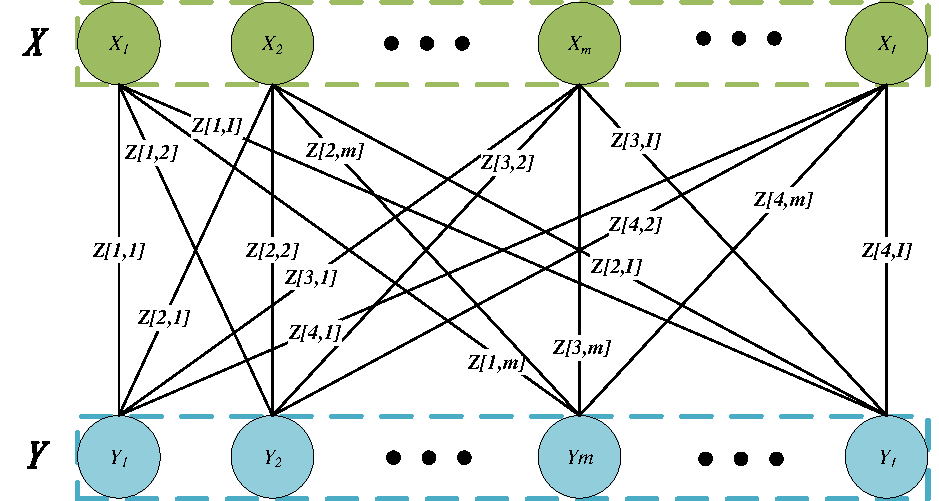
\includegraphics[width=2.5in]{KM1.pdf}
\caption{Bipartite representation of defender--target assignment.}
\label{km}
\end{figure}

The tactical objective is to reduce the expected number of surviving targets. Assigning an
additional capable defender to target $t_j$ multiplies its approximate survival probability
by another failure factor. The resulting capacitated assignment is
\begin{equation}
\label{eq:optimization_formulation}
\begin{aligned}
\min_{\mathbf X}\quad
&J(\mathbf X)=\sum_{j=1}^{N_A}\prod_{i=1}^{N_D}
       \left(1-p_{ij}^{\mathrm{int}}\right)^{X_{ij}}\\
\mathrm{s.t.}\quad
&\sum_{j=1}^{N_A}X_{ij}=1, && i=1,\ldots,N_D,\\
&1\leq\sum_{i=1}^{N_D}X_{ij}\leq L_{\max},
&&j=1,\ldots,N_A,\\
&X_{ij}\in\{0,1\}.&&
\end{aligned}
\end{equation}
The first constraint assigns every defender to exactly one target; the second prevents both
uncovered targets and excessive concentration. A feasible assignment requires
$N_A\leq N_D\leq L_{\max}N_A$.

\subsection{Local IDBO Search and Consensus Bidding}
\label{subsec:idbo_algorithm}

The distributed solution alternates between two interpretable operations. Each defender first
searches for a promising target using locally available engagement information; neighboring
defenders then reconcile conflicting choices by exchanging target-specific bids. Defender
$d_i$ maintains an unconstrained preference vector
$\boldsymbol{\xi}_i\in\mathbb{R}^{N_A}$ and maps it to soft preferences
$\pi_{ij}=\sigma(\xi_{ij})$, where $\sigma(x)=(1+e^{-x})^{-1}$. This separates the
continuous search variable $\xi_{ij}$ from the binary assignment variable $X_{ij}$.

For target $t_j$, let $\widehat n_{ij}=\sum_{\ell\in\mathcal N_i\setminus\{i\}}
\widehat\pi_{\ell j}$ be the assignment load estimated from defender $d_i$'s neighbor set
$\mathcal N_i$. The target-specific utility and aggregate local fitness are
\begin{equation}
\label{eq:local_utility}
\begin{aligned}
u_{ij}(\boldsymbol\xi_i)
 &=\pi_{ij}\bigl(p_{ij}^{\mathrm{int}}+\lambda_A\chi_{ij}\bigr)
 -\lambda_L\pi_{ij}
   \left[\widehat n_{ij}+\pi_{ij}-L_{\max}\right]_{+},\\
\mathcal F_i(\boldsymbol\xi_i)&=\sum_{j=1}^{N_A}u_{ij}(\boldsymbol\xi_i),
\end{aligned}
\end{equation}
where $[x]_{+}=\max(0,x)$ and $\chi_{ij}$ is the combat advantage. The first term favors
interceptable and tactically advantageous targets; the hinge term is inactive below the
estimated capacity and increases only when another defender would oversubscribe that target.

The advantage combines time, relative-velocity compatibility, encounter geometry, and local
competition:
\begin{equation}
\label{eq:adversarial_advantage}
\begin{aligned}
\chi_{ij}={}&
\exp\!\left(-\frac{\Delta t_{ij}}{T_c}\right)
\left[1-\frac{\|\mathbf v_{D_i}-\mathbf v_{T_j}\|_2}{v_c}\right]_{+}
\left[\cos(\vartheta_{ij})\right]_{+}\\
&-\lambda_C\!\sum_{\ell\in\mathcal N_i\setminus\{i\}}
\frac{p_{\ell j}^{\mathrm{int}}}
{p_{ij}^{\mathrm{int}}+p_{\ell j}^{\mathrm{int}}+\varepsilon_{\mathrm{num}}}
\widehat\pi_{\ell j}.
\end{aligned}
\end{equation}
Here, $\Delta t_{ij}$ is the estimated intercept time, $\vartheta_{ij}$ is the encounter
aspect angle, and $T_c$ and $v_c$ are positive normalization constants. The positive-part
operators prevent a large relative-speed mismatch or an unfavorable aspect angle from
producing a negative multiplicative ``advantage.'' The final term lowers the utility of a
target already preferred by capable neighbors.

Rather than presenting four long update equations in succession, we collect the rolling,
dancing, breeding, and stealing operations into one implementation operator:
\begin{equation}
\label{eq:idbo_update}
\boldsymbol\xi_i^{(k+1)}=
\Pi_{\Xi}\!\left[
\mathcal U_{\mathrm{IDBO}}
\bigl(\boldsymbol\xi_i^{(k)},\mathcal F_i,
      \boldsymbol\chi_i^{(k)};k\bigr)\right].
\end{equation}
The four operations respectively perform local exploitation, controlled perturbation, elite
recombination, and preference exchange. Their coefficients decay with assignment iteration
$k$, so early iterations explore broadly and later iterations refine high-utility candidates.
$\Pi_{\Xi}$ clips the latent preferences to their numerical search bounds after every update.
The procedural order and feasibility repair are stated explicitly in Algorithm~\ref{alg:idbo};
the compact form in \eqref{eq:idbo_update} keeps the main physical flow visible.

After local search, defender $d_i$ selects exactly one candidate target,
\begin{equation}
\label{eq:candidate_assignment}
\widetilde X_{ij}^{(k+1)}=
\mathbb I\!\left[j=\underset{r\in\{1,\ldots,N_A\}}{\arg\max}
u_{ir}(\boldsymbol\xi_i^{(k+1)})\right],
\end{equation}
with deterministic index-based tie breaking. Unlike independent thresholding, this mapping
cannot return either zero targets or multiple targets for one defender. The corresponding bid
amplifies targets for which the defender has an above-average combat advantage:
\begin{equation}
\label{eq:bid_formulation}
b_{ij}^{(k+1)}=\widetilde X_{ij}^{(k+1)}u_{ij}
\exp\!\left(\frac{\chi_{ij}-\bar\chi_i}
{s_{\chi,i}+\varepsilon_{\mathrm{num}}}\right),
\end{equation}
where $\bar\chi_i$ and $s_{\chi,i}$ are the mean and standard deviation of
$\{\chi_{ij}\}_{j=1}^{N_A}$.

Each defender stores a local winner set $\mathcal W_{i,j}$ for every target. After receiving
neighbor copies, it retains the highest $L_{\max}$ bids:
\begin{equation}
\label{eq:cbba_update}
\mathcal W_{i,j}^{(k+1)}=\operatorname{Top}_{L_{\max}}
\left(\mathcal W_{i,j}^{(k)}
\cup\!\bigcup_{\ell\in\mathcal N_i}\mathcal W_{\ell,j}^{(k)}
\cup\{(d_i,b_{ij}^{(k+1)})\}\right).
\end{equation}
Because only the selected target receives a nonzero bid, the winner sets enforce the target
capacity without destroying the one-target-per-defender interpretation. A defender displaced
from a full winner set removes that target from its local candidate and searches/bids again in
the next iteration.

\begin{figure}[!t]
\centering
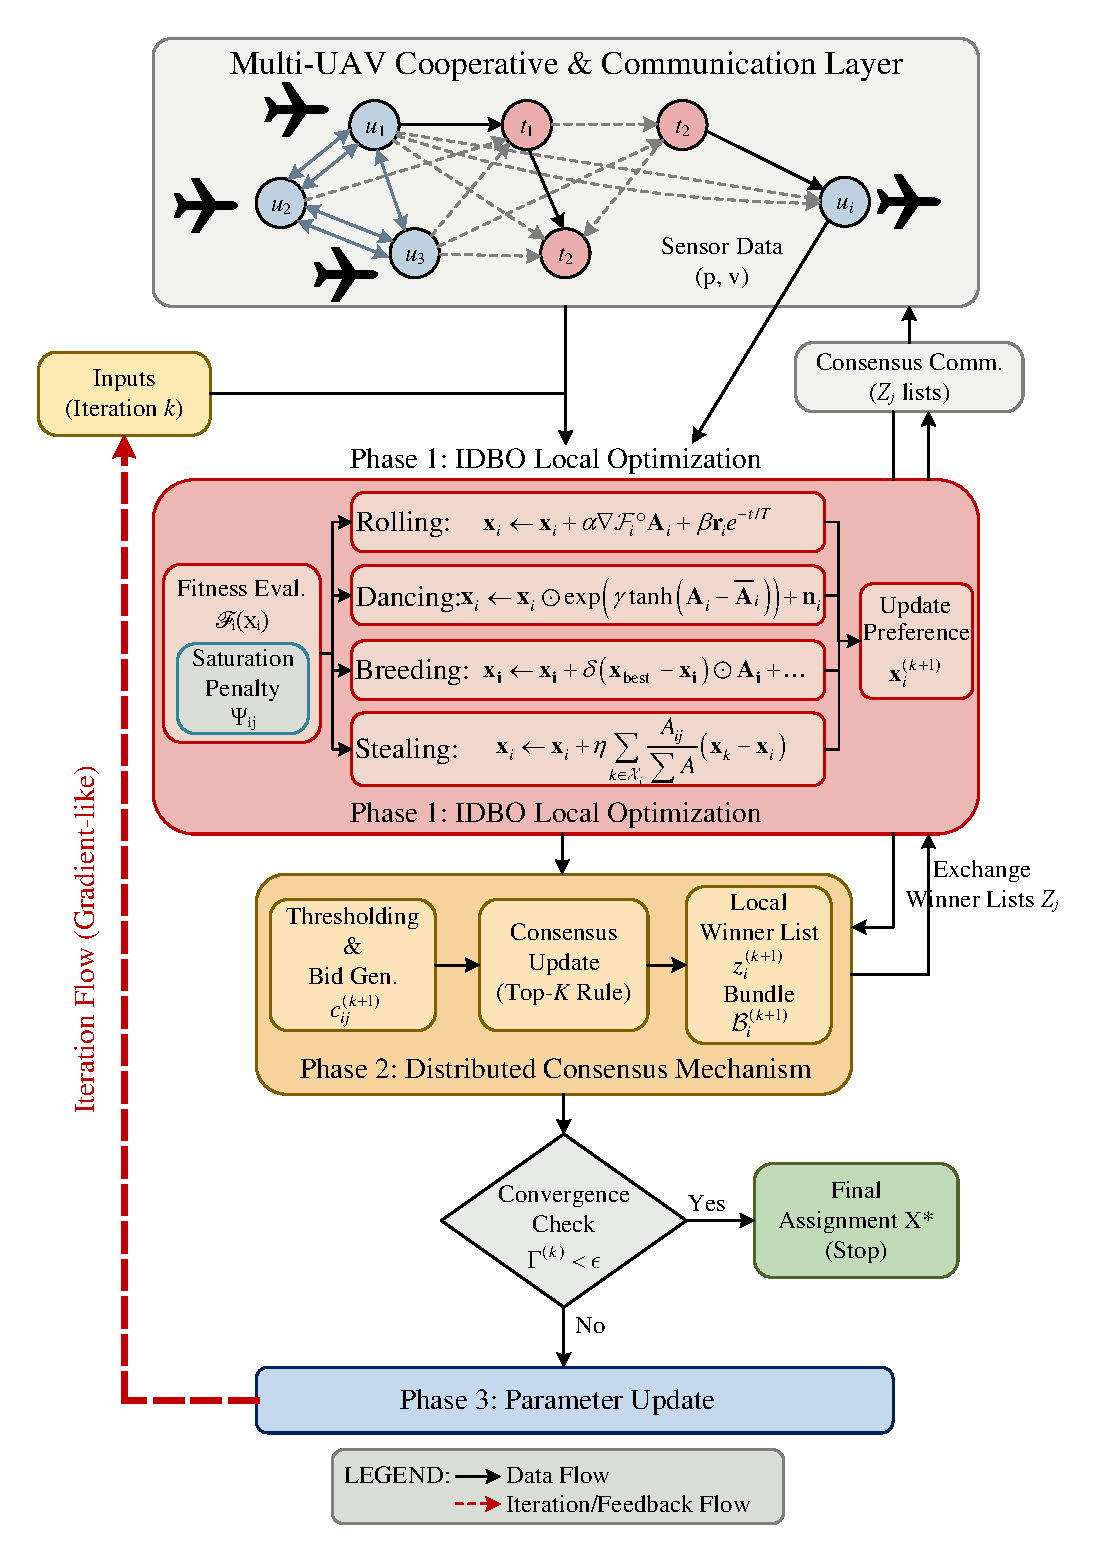
\includegraphics[width=3.2in]{assignment.pdf}
\caption{Distributed IDBO assignment flow: local preference search, one-hot candidate
selection, top-$L_{\max}$ consensus bidding, and engagement-information update.}
\label{fig:idbo_flowchart}
\end{figure}

Let $\mathbf W_i^{(k)}=\{\mathcal W_{i,j}^{(k)}\}_{j=1}^{N_A}$ and let
$\mathcal E$ denote the communication edges. The normalized pairwise disagreement is
\begin{equation}
\label{eq:convergence}
\Gamma^{(k)}=\frac{1}{|\mathcal E|}
\sum_{(i,\ell)\in\mathcal E}
\mathbb I\!\left[\mathbf W_i^{(k)}\neq\mathbf W_{\ell}^{(k)}\right]
\leq\varepsilon_{\mathrm{con}}.
\end{equation}
This definition directly counts communication links whose winner information is inconsistent;
it is zero when all neighboring defenders agree.

\subsection{Convergence Scope and Computational Cost}
\label{subsec:convergence_equilibrium}

The convergence statement concerns agreement of the distributed assignment process for a
fixed engagement snapshot, not global optimality of the nonconvex problem in
\eqref{eq:optimization_formulation}. We assume that the defender/target sets are fixed during
one assignment round, the communication graph is connected with bounded delay, bids use
deterministic tie breaking, and accepted local candidates are retained only when they improve
the projected local fitness. Under these conditions, each target's highest bids propagate
through the connected graph in finitely many communication rounds. Since the binary feasible
set and the winner sets are finite, the deterministic local-search/consensus process reaches a
locally stable fixed point unless the prescribed iteration limit is met first. This guarantees
consistent winner information; it does not establish a global optimum or an
$\varepsilon$-Nash bound.

For one defender and one assignment iteration, evaluating a population of $N_{\mathrm{pop}}$
candidates over $N_A$ targets costs $O(N_{\mathrm{pop}}N_A)$, exchanging target bids costs
$O(N_A|\mathcal N_i|)$, and updating the advantage costs $O(N_A)$. For $K_{\mathrm{IDBO}}$
iterations, these terms are multiplied by $K_{\mathrm{IDBO}}$; per-defender memory is
$O(N_{\mathrm{pop}}N_A+N_A)$.

\begin{algorithm}[!t]
\caption{Distributed Consensus-Based IDBO Target Assignment}
\label{alg:idbo}
\footnotesize
\begin{algorithmic}[1]
\REQUIRE $\mathcal D$, $\mathcal T$, $p_{ij}^{\mathrm{int}}$, neighbor sets
$\mathcal N_i$, capacity $L_{\max}$, tolerance $\varepsilon_{\mathrm{con}}$,
maximum iteration $K_{\max}$
\ENSURE Consensus assignment $\mathbf X^{*}$
\STATE Initialize $\boldsymbol\xi_i$, bids $b_{ij}$, and local winner sets
$\mathcal W_{i,j}$ for every defender
\FOR{$k=0$ to $K_{\max}-1$}
    \FOR{each defender $d_i$}
        \STATE Evaluate $p_{ij}^{\mathrm{int}}$, $\chi_{ij}$, and
        $u_{ij}$ from the current engagement snapshot
        \STATE Update $\boldsymbol\xi_i$ with the IDBO operator in
        \eqref{eq:idbo_update} and project it to the search bounds
        \STATE Form the one-hot candidate $\widetilde{\mathbf X}_{i,:}$ using
        \eqref{eq:candidate_assignment} and compute its bid using
        \eqref{eq:bid_formulation}
        \STATE Exchange $\{\mathcal W_{i,j}\}_{j=1}^{N_A}$ with neighbors and
        retain top-$L_{\max}$ bids using \eqref{eq:cbba_update}
        \STATE If displaced, remove the conflicting candidate before the next search step
    \ENDFOR
    \STATE Compute $\Gamma^{(k+1)}$ using \eqref{eq:convergence}
    \IF{$\Gamma^{(k+1)}\leq\varepsilon_{\mathrm{con}}$}
        \STATE \textbf{break}
    \ENDIF
\ENDFOR
\STATE Construct $\mathbf X^{*}$ from the agreed winner sets and apply a deterministic
feasibility repair if an uncovered target remains
\end{algorithmic}
\end{algorithm}
